\chapter{Le triphasé}
\section{Notations - Conventions}
	
\subsection{Conventions}
\begin{wrapfigure}[10]{l}{3cm}
	\vspace{-5mm}
	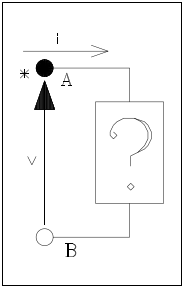
\includegraphics[scale=0.4]{ch1/image1.png}
	\captionof{figure}{ }
\end{wrapfigure}
La convention \textit{récepteur} sera celle utilisée : la puissance 
sera positive lorsqu'elle sera absorbée par la machine. Pour une 
source de tension $v$, c'est le contraire : le courant - défini par 
les charges positives -sera dans le sens de la flèche.\\

L'astérisque 
marque ainsi la borne d'entrée d'un dipôle ou un cercle plein.\\
	
Dernière convention : la flèche de tension désigne la borne à 
laquelle il faut appliquer une tension positive pour faire circuler 
un courant positif.
	
\subsection{Notations}
\begin{tabular}{ll}
	$a = a(t)$                      & : valeur instantanée                                             \\
	$\underline{a}(t)$              & : valeur instantanée complexe ; vecteur tournant                 
	dont la projection sur un axe de\\
	                                & \ \ \  référence fournit la valeur instantanée                 
	d'une grandeur sinusoïdale de pulsation $\omega$ ; \\
	                                & \ \ \	$a(t) = \Re(                                                
	\underline{a}(t))$\\
	$\underline{A} = A\angle\alpha$ & : nombre complexe de module $A$ et                                
	d'argument $\alpha$.\\
	$A_M$                           & : valeur de crête ou maximale dans le temps : $A_M = a \sqrt{2}$ \\
	$\overline{A}$                  & : vecteur spatial de module $A$                                   \\
	$A^M$                           & : valeur maximale d'une grandeur variant dans l'espace            \\
	$i_{ab}$                        & : courant circulant de $A$ vers $B$ ($A\rightarrow B$)            \\
	$v_{ba} = v_a-v_b$              & : potentiel de $A$ par rapport à $B$ ($B \rightarrow A$)         
\end{tabular}

\section{Rappel de quelques notions relatives aux courants alternatifs}
\subsection{Représentation des fonctions sinusoïdale du temps}
Un telle grandeur, de pulsation $\omega$ est représentée par :
\begin{equation}
	\begin{array}{lll}
		v & = V_M\cos(\omega t + \xi_v)       & \text{où $V_M$ est la valeur de crete} \\
		  & = V\sqrt{2}\cos(\omega t + \xi_v) & \text{où $V$ est la valeur efficace}   
	\end{array}
\end{equation}
Ceci peut s'écrire 
\begin{equation}
	\begin{array}{ll}
		v & = \Re (V\sqrt{2}\cos(\omega t + \xi_v) + jV\sqrt{2}\sin(\omega t + \xi_v)) \\
		  & = \Re (V\sqrt{2}e^{j(\omega t + \xi_v})                                    
	\end{array}
\end{equation}
La \textbf{valeur instantannée complexe} $\overline{v}$ est définie par \\
\begin{wrapfigure}[12]{r}{5cm}
	\vspace{-15mm}
	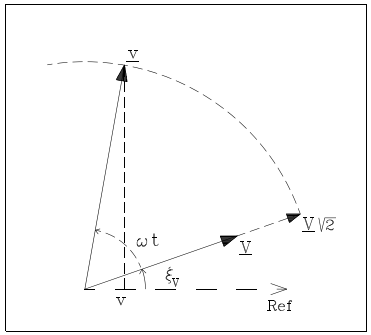
\includegraphics[scale=0.4]{ch1/image2.png}
	\captionof{figure}{ }
\end{wrapfigure}
\begin{equation}
	\begin{array}{ll}
		\overline{v} & = V \sqrt{2}e^{j(\omega t + \xi_V)} \\
		             & = V e^{j\xi_V}\sqrt{2}e^{j\omega t} 
	\end{array}
\end{equation}
où le \textbf{phaseur} $\underline{V}$ est 
\begin{equation}
	\underline{V} = Ve^{j\xi_V}
\end{equation}
Dans le plan de Gauss $\overline{V}$ a un module valant la valeur efficace 
de la grandeur et un argument valant $\xi_V$, c'est un vecteur \textsc{fixe}.
La valeur instantanée complexe $\underline{v}$ a un module $V\sqrt{2}$ et est 
décalée de $V\sqrt{2}$ par rapport à $\overline{V}$ : c'est un vecteur 
\textsc{tournant} (à $\omega$). On obtient la valeur instantanée en projetant 
la valeur instantanée complexe sur l'axe réel : $v = \Re(\underline{v})$.\\
	
Les déphasages entre grandeurs sont constants : on considère comme référence un 
courant $\underline{I}$ et on définit l'argument de la tension par rapport à 
celui-ci à l'aide de l'\textbf{angle de charge} $\varphi$.
	
\begin{center}
	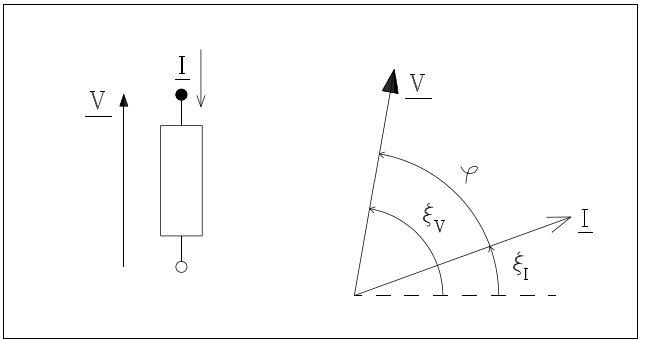
\includegraphics[scale=0.4]{ch1/image3.png}
	\captionof{figure}{ }
\end{center}	
		
Si l'on applique la tension $\underline{V} = V\angle \xi_V$ à une impédance 
$\underline{Z} = R + jX = Z\angle \xi$, le courant vaut 
\begin{equation}
	\underline{I} = \frac{\underline{V}}{\underline{Z}} = \frac{V}{Z}\angle 
	\xi_V-\xi
\end{equation}
On remarque avec l'argument du courant qu'une impédance inductive ($X>0, 
\xi <0$) déphase le courant en arrière par rapport à la tension et l'inverse 
pour une impédance capacitive.
	
	
\subsection{Représentation de la puissance}
\subsubsection{Puissance active}
Cherchons à calculer la puissance de $A$ vers $B$ au point $X$. Nous 
avons $v = V_M\cos(\omega t +\xi_V)$ et $i = I_M\cos(\omega t + \xi_I)$. 
La valeur instantanée de la puissance vaut :
\begin{equation}
	\begin{array}{ll}
		p & = v\ i                                                               \\
		  & = V_MI_M\cos(\omega t +\xi_V)\cos(\omega t +\xi_I)                   \\
		  & = \frac{V_MI_M}{2}(\cos(\xi_V-\xi_I) + \cos(2\omega t +\xi_V+\xi_I)) \\
		  & = \underbrace{VI \cos\varphi}_{1} + \underbrace{VI \cos(2\omega t +  
		\xi_V+\xi_I)}_{2}
	\end{array}
\end{equation}
Cette expression contient deux termes :
\begin{enumerate}
	\item La puissance active, c'est la valeur moyenne de $p$.
	\item Un terme pouvant causer des vibrations indésirables.
\end{enumerate}
La \textbf{puissance utile} est celle correspondant à un travail 
effectué :
\begin{equation}
	P = VI \cos\varphi
\end{equation}
		
\subsubsection{Puissance apparente}
Par définition
\begin{equation}
	\begin{array}{ll}
		\underline{S} & \equiv \underline{V}\underline{I^*} \\
		              & = VI \angle \xi_V-\xi_I             \\
		              & = VI\angle\varphi                   
	\end{array}
\end{equation}
Si la tension est constante, la puissance apparente est proportionnelle 
au courant.
\begin{center}
	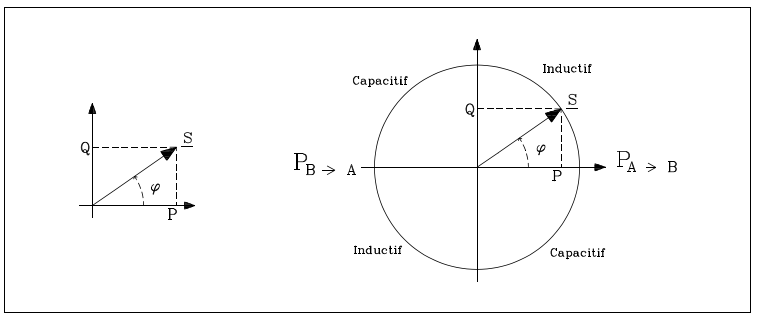
\includegraphics[scale=0.4]{ch1/image4.png}
	\captionof{figure}{ }
\end{center}	
		
\subsubsection{Puissance réactive}
Dans l'expression $P = VI \cos\varphi = \Re(\underline{S})$, on définit la 
\textbf{puissance réactive} :
\begin{equation}
	Q = VI\sin\varphi = \Im(\underline{S})
\end{equation}
tel que $\underline{S} = P+jQ$.\\
Si $P>0, Q>0$ si $\varphi>0$ c'est à dire que la charge est inductive.\\
Si $P>0, Q<0$ si $\varphi<0$ c'est à dire que la charge est capacitive.\\
			
La puissance réactive ne correspond à aucun travail effectif et est une 
notion difficile à saisir. Retenons juste que sa circulation amène des 
pertes et des chutes de tension. Cette puissance n'apparaît que si la 
charge est réactive, c'est-à-dire peut stocker de l'énergie\footnote{Voir 
1.2-14 du syllabus pour une image intuitive}.
\newpage		
\section{Caractéristiques d'un système polyphasé}
\subsection{Modes de couplage des circuits polyphasés}
\begin{wrapfigure}[13]{l}{8.5cm}
	\vspace{-8mm}
	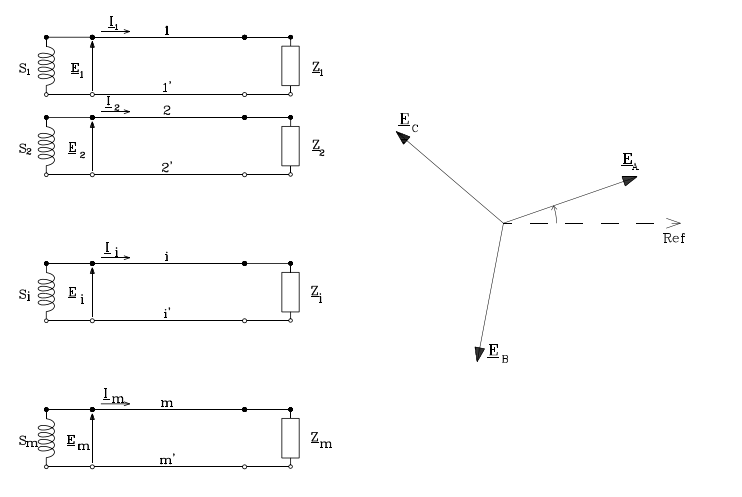
\includegraphics[scale=0.34]{ch1/image5.png}
	\captionof{figure}{ }
\end{wrapfigure}	
Soit $m$ sources électrique indépendantes $S_1, S_2,\dots,S_m$ dont les tensions 
ont la même valeur efficace et sont déphasées de $2\pi/m$ : système $m-$phasé 
équilibré d'ordre direct :
\begin{equation}
	\underline{E_i} = E_{1} \langle -(i-1)\frac{2\pi}{m}
\end{equation}


\textsc{Convention :} la phase 2 est située en arrière de la phase 1 et la 
phase 3 en arrière de la phase 2 (en arrière signifie "[...] dans le temps").\\
	
Ci-dessus, un schéma de principe pour un tel système. Chacun des enroulements d'
induit est raccordé par deux fils, il faudrait donc $2m$ conducteurs. Il existe 
deux moyens d'économiser le métal conducteur :
	
\subsubsection{a. Couplage en étoile avec fil neutre}
\begin{wrapfigure}[12]{r}{8cm}
	\vspace{-5mm}
	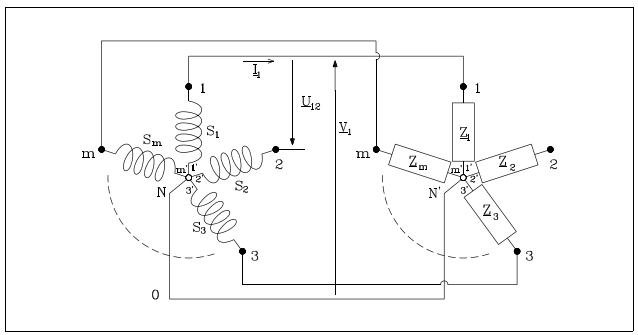
\includegraphics[scale=0.4]{ch1/image6.png}
	\captionof{figure}{ }
\end{wrapfigure}
L'idée est d'utiliser un conducteur de retour commun à tous les circuits 
en réunissant les extrémités. On appelle $O$, le fil neutre parcouru par 
la somme des courants débités par toutes les sources. Nécessitant $m+1$ 
fil de ligne, il s'agit du couplage \textit{étoilé avec fil neutre}.\\
		
La \textbf{tension simple} (ou de \textbf{phase}) d'un conducteur est 
la différence de potentiel entre le conducteur et le neutre. Par 
exemple : $\underline{V}_1 = \underline{V}_1-\underline{V}_0$. La 
\textbf{tension composée} (ou \textbf{entre phases}) est la différence 
de potentiel entre deux conducteurs. Par exemple : $\underline{U}_{12} = 
\underline{V}_2-\underline{V}_1$.
		
		
\subsubsection{b. Couplage en étoile sans fil neutre}
Si toutes les impédances sont identiques, le circuit est équilibre et 
la somme des courants de ligne est nulle : $\sum_{i=1}^m i_i=0$. Comme 
le neutre n'est plus parcouru, on peut le supprimer. Le point $N'$, 
neutre, possède le même potentiel que le point $N$ par symétrie : $N$ 
est un point neutre artificiel. Cette installation comporte $m$ fils.\\
\begin{wrapfigure}[6]{l}{8.5cm}
	\vspace{-8mm}
	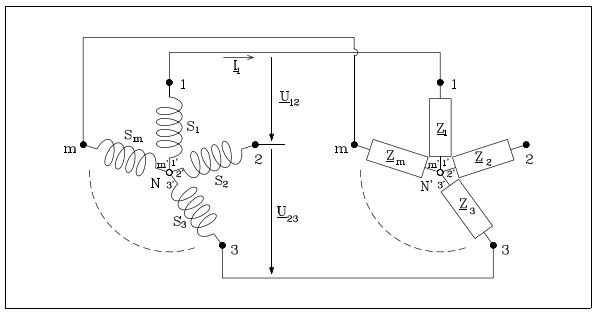
\includegraphics[scale=0.4]{ch1/image7.png}
	\captionof{figure}{ }
\end{wrapfigure}		
Spoil : si les charges sont déséquilibrées on peut conserver ce montage 
mais la tension de $N' \neq N$. Cherchons maintenant les relations liant 
tension et phase.\\
Soit $\underline{V}_1, \underline{V}_2$ les tensions mesurées entre 
neutre de phase consécutives 1 et 2. Par symétries, elle sont égales 
en tension efficace mais déphasées de $2\pi/m$ radians. Si $\underline{
V_1}$ est la référence :
\begin{equation}
	\begin{array}{ll}
		\underline{V_1} & = V\angle 0               \\
		\underline{V_2} & = V\angle -\frac{2\pi}{m} 
	\end{array}
\end{equation}
Le phaseur de la tension mesurée entre les phases 1 et 2 s'écrit
\begin{equation}
	\underline{U}_{12} = \underline{V_2}-\underline{V_1}
\end{equation}
On voit que\footnote{??} 
\begin{equation}
	\begin{array}{ll}
		\underline{U}_{12} & = 2\underline{V}_1\sin \frac{\pi}{m}e^{-j\left( 
		\frac{\pi}{m}+\frac{\pi}{2}\right)}\\
		U_{12}             & = 2V_1\sin\frac{\pi}{m}                         
	\end{array}
\end{equation}
		
La puissance transportée par une ligne équilibrée vaudra alors 
\begin{equation}
	P = \Re(m \underline{V}_1\underline{I_1}^*) = mV_1I_1\cos\varphi
\end{equation}
		
Si le point neutre n'est pas accessible, la seule tension mesurable 
est $U_{12}$. En remplaçant dans $P$, la valeur $V_1$ tirée de 
$U_{12}$ :
\begin{equation}
	P = \frac{m}{2\sin\frac{\pi}{m}}U_{12}I_1\cos\varphi
\end{equation}
\textbf{Attention :} $\varphi$ est le déphasage entre tension simple 
et courant et rien d'autre!
		
		
\subsubsection{c. Couplage en polygone}
\begin{wrapfigure}[10]{l}{8.5cm}
	\vspace{-5mm}
	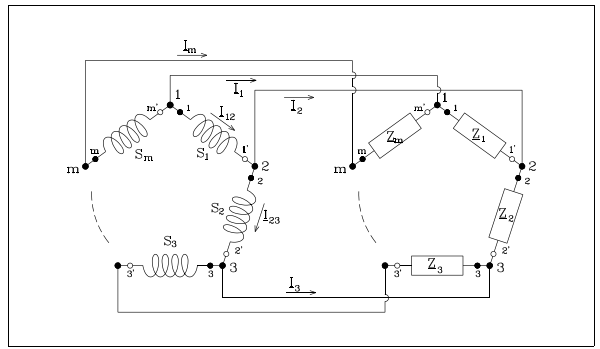
\includegraphics[scale=0.4]{ch1/image8.png}
	\captionof{figure}{ }
\end{wrapfigure}		
On peut connecter la sortie de chacune des phases du générateur à 
l'entrée de la phase contiguë et de même pour le récepteur. La somme 
des f.e.m. alternatives équilibrées engendrées dans les phases du 
générateurs étant nulles, on peut les connecter pour former un 
\textbf{polygone fermé} (le courant ne circulera pas). On aura pour ça
besoin de $m$ conducteurs distincts.\\
\ \\
\\

Soit $\underline{I}_{12}$ et $\underline{I}_{23}$ les courants qui 
circulent dans deux phases consécutives du générateur et $\underline{I}_
2$, le courant traversant la ligne commune. Par Kirchoff :
\begin{equation}
	\underline{I}_2 = \underline{I}_{12}-\underline{I}_{23}
\end{equation}
Or $\underline{I}_{12}$ et $\underline{I}_{23}$  sont égaux en 
grandeur et entre eux se trouve un angle de $2\pi/m$. Par les 
relations vectorielles :
\begin{equation}
	\underline{I}_2 = \underline{I}_{12}\sin\frac{\pi}{m}e^{-j\left(\frac{
		\pi}{m}-\frac{\pi}{2}\right)}
\end{equation} 
		
		
\subsubsection{d. Puissance électrique transportée par une ligne}
Cette puissance s'exprime par 
\begin{equation}
	P = \Re(m\underline{U}_{12}\underline{I}_{12}^*) = mU_{12}I_{12}\cos
	\varphi = \frac{m}{2\sin\frac{\pi}{m}}U_{12}I_1\cos\varphi
\end{equation}
La puissance transmise est bien indépendante du mode de couplage du 
générateur / récepteur.
		
\subsection{Cas particulier de couplage : le système triphasé}
Les trois tensions seront égales, mais décalées de $2\pi/3$. On pourra 
les exprimer :
\begin{equation}
	\begin{array}{ll}
		e_A & = E\sqrt{2}\cos(\omega t +\xi_V)                  \\
		e_B & = E\sqrt{2}\cos(\omega t +\xi_V - \frac{2\pi}{3}) \\
		e_C & = E\sqrt{2}\cos(\omega t +\xi_V + \frac{2\pi}{3}) 
	\end{array}
\end{equation}
Définissions l'opérateur de déphasage $\underline{\alpha} = \angle \frac{2
	\pi}{3} = -\frac{1}{2}+j\frac{\sqrt{3}}{2}$ tel que $\underline{E_B} = 
\underline{\alpha}^2\underline{E_A}$ et $\underline{E_C} = \underline{\alpha}
\underline{E_A}$.\\
Des relations intéressantes sont reprises en (1.3-19). Notons juste que 
la somme des courants est bien nulle : $1+\underline{\alpha}+\underline{
	\alpha}^2 = 0$.
		
\subsubsection{Couplage en étoile}
\begin{wrapfigure}[8]{l}{8.5cm}
	\vspace{-5mm}
	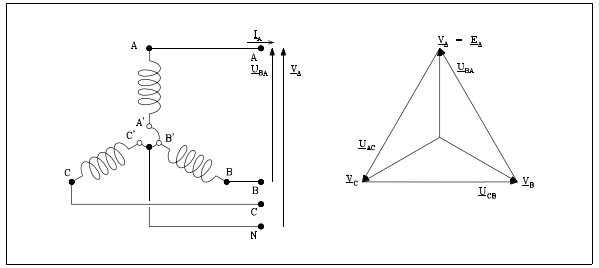
\includegraphics[scale=0.4]{ch1/image9.png}
	\captionof{figure}{ }
\end{wrapfigure}
On peut relier $A',B',C'$ en un point neutre $N$ et $A,B,C$ sont les 
sorties de l'alternateur raccordées aux fils de lignes. Les tensions 
sont égales aux f.e.m. engendrées et sont dès lors également un 
système triphasé équilibre. Pour les tensions composées, on les 
obtient par composition vectorielle :
\vspace{1cm}
\begin{equation}
	\begin{array}{llll}
		\underline{U}_{BA} & = \underline{V}_A-\underline{V}_B & = \underline{V}_A 
		(1-\underline{\alpha}^2) &= \underline{V_A}\sqrt{3}\angle\frac{\pi}{6}\\
		\underline{U}_{CB} & = \underline{V}_B-\underline{V}_C & = \underline{V}_A 
		(\underline{\alpha}^2-\underline{\alpha}) &= \underline{V_A}\sqrt{3}\angle
		-\frac{\pi}{2}		\\
		\underline{U}_{AC} & = \underline{V}_C-\underline{V}_A & = \underline{V}_A 
		(\underline{\alpha}-1) &= \underline{V_A}\sqrt{3}\angle\frac{5\pi}{6}
	\end{array}
\end{equation}
$\Longrightarrow U = V\sqrt{3}$. La puissance est donnée par $P = 3VI
\cos\varphi$.
		
\subsubsection{Couplage en triangle}
La borne $C'$ de la phase $C$ est reliée à la borne $A$ de la phase 
$A$ de la ligne :
\begin{equation}
	\begin{array}{ccc}
		\underline{U}_{BA} = \underline{E_A},\quad & \quad \underline{U}_{CB} =                  
		\underline{E_B}, \quad                     & \quad \underline{U}_{AC} = \underline{E_C}. 
	\end{array}		
\end{equation}
Le centre de gravité du triangle des tensions peut représenter le 
potentiel d'un neutre fictif $N$ pour définir un système de tension 
simple. Pour les résultats, voir page 1.23.
\begin{center}
	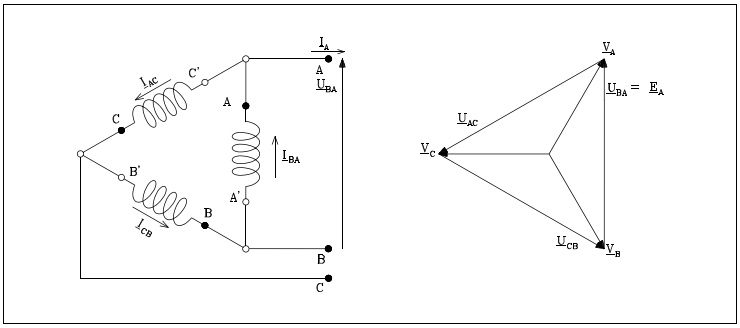
\includegraphics[scale=0.4]{ch1/image10.png}
	\captionof{figure}{ }
\end{center}		
		
		
\subsection{Influence des harmoniques dans les circuits polyphasés}
Les tensions ne sont pas toujours sinusoïdales. On peut décomposer une courbe 
périodique par une somme de sinusoïdes. Ici, les fonctions du temps 
présentent deux alternances identiques, c'est à dire que superposables par 
retournement :
\begin{equation}
	f(t+\frac{T}{2}) = -f(t)
\end{equation}
Une fonction qui satisfait ceci n'a que des coefficients de Fourier impairs 
dans son développement. Intéressons-nous au cas du triphasé. \\
Soit la f.e.m. $e_A$ sous la forme d'une série de Fourier :
\begin{equation}
	e_A = \sum_{i=1}^\infty A_i\cos(i\omega t + \xi_i)
\end{equation}
avec $i$ impair. Les f.e.m. développées par les phases $e_B$ et $e_C$ s'
obtiennent en remplaçant $\omega t$ par $\omega t - 2\pi/3$ et $\omega t 
+2\pi/3$.\\
Cas du couplage triangle et étoile vu en cours ? Passé ici.
	
\subsection{Mesure de la puissance dans les circuits polyphasés}
\subsubsection{Méthode des $m$ wattmètres - Circuit sans fil neutre}
\begin{wrapfigure}[12]{r}{5cm}
	\vspace{-11mm}
	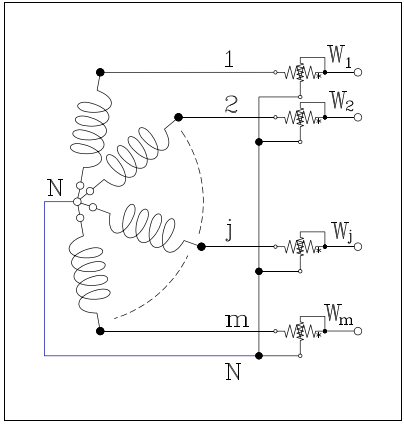
\includegraphics[scale=0.4]{ch1/image11.png}
	\captionof{figure}{ }
\end{wrapfigure}
Soit un circuit polyphasé à $m$ phases sans fil neutre disposé en 
étoile au neutre accessible. Pour mesurer la puissance, on introduit 
dans chaque ligne un wattmètre (connecté entre la phase et le neutre). 
La puissance totale est alors la somme des $m$ mesures. Si le système 
est équilibré, tous les wattmètres indiqueront la même puissance. La 
puissance débitée vaut alors
\begin{equation}
	p = \sum_{j=1}^m W_j = \sum_{j=1}^m (v_j-v_n)i_j = \sum_1^m v_ji_j -
	v_n\sum_1^m i_j
\end{equation}
Si le neutre n'est pas connecté, la somme des courants est nulle et le 
potentiel de $N$ peut être remplacé par celui d'un point quelconque. Les 
indications de chaque wattmètre seront modifiées, mais pas leur somme.
		
\subsubsection{Méthode des $m-1$ wattmètres}
Comme on peut choisir $N'$ quelconque, portons le retour des wattmètres 
sur la $m^{ème}$ phase. Le wattmètre $m$ ne sert plus à rien car la 
tension à ses bornes est annulée : il ne faut plus que $m-1$ wattmètres.
		
\subsection{Facteur de puissance}
Il faut avant tout un équilibre des phases et dans ce cas, ce facteur n'est 
autre que $\cos\varphi$ de l'un des circuit : 
\begin{equation}
	P_A = V_AI_A\cos\varphi
\end{equation}
La puissance totale débitée vaut alors $P = mP_A$. Quand les phases sont 
équilibrés, on peut toujours écrire
\begin{equation}
	P = \sum_1^m V_jI_j\cos\varphi_j
\end{equation}
Comme $\varphi_j$ peut être différent dans chacune des phases : on ne peut 
plus définir un $\cos\varphi$ global mais un facteur de puissance :
\begin{equation}
	FP = \frac{P}{S} = \frac{P}{\sqrt{P^2+Q^2}}
\end{equation}
Notons que $\tan\varphi = \frac{Q}{P}$.
	
\subsection{Mesure de la puissance dans les circuits triphasés}
\subsubsection{a. Circuit triphasé étoile avec fil neutre}
\begin{wrapfigure}[5]{l}{4.5cm}
	\vspace{-5mm}
	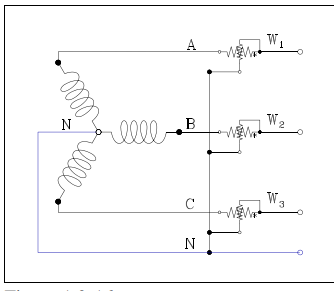
\includegraphics[scale=0.35]{ch1/image12.png}
	\captionof{figure}{ }
\end{wrapfigure}

Soit un alternateur triphasé connecté en étoile avec un neutre $N$ 
débitant sur un circuit triphasé étoile ou triangle. Quel que soit 
le déséquilibre, la puissance sera donnée par la somme des valeurs 
des trois wattmètres. Le facteur de puissance est alors le rapport 
entre la puissance totale mesurée et la puissance apparente donnée 
par $V_iI_i$.\\
\\	
\subsubsection{b. Circuit triphasé sans fil neutre}
\begin{wrapfigure}[8]{r}{4.5cm}
	\vspace{-5mm}
	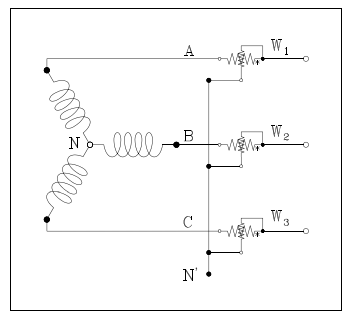
\includegraphics[scale=0.35]{ch1/image13.png}
	\captionof{figure}{ }
\end{wrapfigure}		
Cette fois-ci on n'a pas de neutre. On peut utiliser la méthode des 
trois wattmètres : la borne d'entrée de chaque wattmètre est connectée 
à chacun des fils de lignes et toutes les bornes de sorties sont 
connectées ensembles de façon à former un point neutre artificiel $N'$. 
Si les wattmètres sont identiques, alors $N'=N$. Sinon, le potentiel 
de $N'$ est quelconque mais la puissance totale est la somme de tous 
les wattmètres. Si le circuit est équilibré, une seule mesure est 
suffisante.\\
		
				
		
\textsc{Méthode des deux wattmètres}\\
On insère les wattmètres en $A$ et $B$ et leur sortie, commune 
en $C$.\\
Si le circuit est parfaitement équilibré d'ordre \textit{direct}, 
la tension de la phase $C$ retarde de $2\pi/3$ sur celle de $B$ 
qui elle même retarde de $2\pi/3$ sur celle de $A$. On a alors
\begin{equation}
	\begin{array}{lll}
		\underline{V}_A    & = V \angle 0                                  \\
		\underline{V}_B    & = V\angle-\frac{2\pi}{3}                      \\
		\underline{V}_C    & = V\angle\frac{2\pi}{3}                       \\
		\underline{I}_A    & = I\angle-\varphi                             \\
		\underline{I}_B    & = I\angle-\varphi-\frac{2\pi}{3}              \\
		\underline{I}_C    & = I\angle-\varphi+\frac{2\pi}{3}              \\
		\underline{U}_{CA} & = \underline{V}_A-\underline{V}_C = V\sqrt{3} 
		\angle-\frac{\pi}{6}\\
		\underline{U}_{CB} & = \underline{V}_B-\underline{V}_C = V\sqrt{3  
		}\angle-\frac{\pi}{2}			
	\end{array}
\end{equation}
\begin{center}
	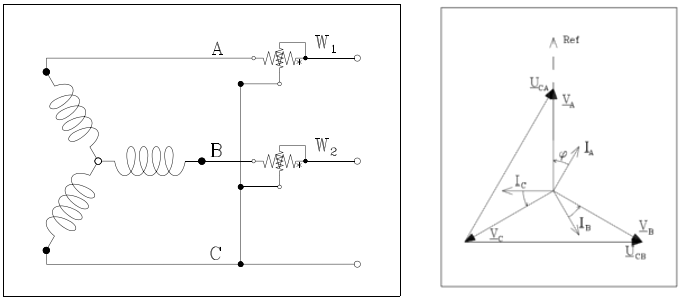
\includegraphics[scale=0.5]{ch1/image14.png}
	\captionof{figure}{ }
\end{center}
Les indications des deux wattmètres vaudront alors forcément
\begin{equation}
	\begin{array}{lll}
		W_1 & = \Re(\underline{U}_{CA}\underline{I_A^*}) & = UI\cos(-\frac{\pi}{           
		6}+\varphi)\\
		W_2 & = \Re(\underline{U}_{CB}\underline{I_B^*}) & = UI\cos(-\frac{\pi}{           
		2}+\varphi+\frac{2\pi}{3})	\\
		    &                                            & = UI\cos(\frac{\pi}{6}+\varphi) 
	\end{array}
\end{equation}
			
La puissance totale vaut évidemment 
\begin{equation}
	P = W_1+W_2 = \sqrt{3}UI\cos\varphi
\end{equation}
		
		
		
		
		
		
		
		
		
		
		
		
		
		
		
		
		
		
